%============================================================================%
%
%       DOCUMENT DEFINITION
%
%============================================================================%

%we use article class because we want to fully customize the page and dont use a cv template
\documentclass[10pt,A4]{article}        


%----------------------------------------------------------------------------------------
%       ENCODING
%----------------------------------------------------------------------------------------

%we use utf8 since we want to build from any machine
\usepackage[utf8]{inputenc}             
\usepackage[ngerman]{babel}

%----------------------------------------------------------------------------------------
%       LOGIC
%----------------------------------------------------------------------------------------

% provides \isempty test
\usepackage{xifthen}

%----------------------------------------------------------------------------------------
%       FONT
%----------------------------------------------------------------------------------------

% some tex-live fonts - choose your own

%\usepackage[defaultsans]{droidsans}
%\usepackage[default]{comfortaa}
%\usepackage{cmbright}
%\usepackage[default]{raleway}
%\usepackage{fetamont}
%\usepackage[default]{gillius}
\usepackage[light,math]{iwona}
%\usepackage[thin]{roboto} 

% set font default
\renewcommand*\familydefault{\sfdefault}        
\usepackage[T1]{fontenc}

% more font size definitions
\usepackage{moresize}           

\usepackage{fontawesome}

%----------------------------------------------------------------------------------------
%       PAGE LAYOUT  DEFINITIONS
%----------------------------------------------------------------------------------------

%debug page outer frames
%\usepackage{showframe}                 


%define page styles using geometry
\usepackage[a4paper]{geometry}          

% for example, change the margins to 2 inches all round
\geometry{top=1cm, bottom=-.6cm, left=0.4cm, right=1cm}         


%less space between header and content
\setlength{\headheight}{-5pt}           


%customize entries left, center and right
%\lhead{}
%\chead{ \small{Jan Küster  $\cdot$ Consultant and Software Engineer $\cdot$  Bremen, Germany  $\cdot$  \textcolor{sectcol}{\textbf{info@jankuester.com}}  $\cdot$ +49 176 313 *** **}}
%\rhead{}


%indentation is zero
\setlength{\parindent}{0mm}

%----------------------------------------------------------------------------------------
%       TABLE /ARRAY DEFINITIONS
%---------------------------------------------------------------------------------------- 

%for layouting tables
\usepackage{multicol}                   
\usepackage{multirow}

%extended aligning of tabular cells
\usepackage{array}

\newcolumntype{x}[1]{%
>{\raggedleft\hspace{0pt}}p{#1}}%


%----------------------------------------------------------------------------------------
%       GRAPHICS DEFINITIONS
%---------------------------------------------------------------------------------------- 

%for header image
\usepackage{graphicx}

%for floating figures
\usepackage{wrapfig}
\usepackage{float}
%\floatstyle{boxed} 
%\restylefloat{figure}

%for SVGs
\usepackage{svg}

%for drawing graphics           
\usepackage{tikz}                               
\usetikzlibrary{shapes, backgrounds,mindmap, trees}


%----------------------------------------------------------------------------------------
%       Color DEFINITIONS
%---------------------------------------------------------------------------------------- 
\usepackage{transparent}
\usepackage{color}

%accent color
\definecolor{complcol_alt}{RGB}{242,182,97}
\definecolor{complcol}{RGB}{242,109,97}

%dark background color
\definecolor{bgcol}{RGB}{110,110,110}

%light background / accent color
\definecolor{softcol}{RGB}{225,225,225}

%\definecolor{sectcol}{RGB}{0,120,150}
\definecolor{sectcol}{RGB}{97, 194, 242}


%============================================================================%
%
%
%       DEFINITIONS
%
%
%============================================================================%

% returns minipage width minus two times \fboxsep
% to keep padding included in width calculations
\newcommand{\mpwidth}{\linewidth-\fboxsep-\fboxsep}
        

%----------------------------------------------------------------------------------------
%       ARROW GRAPHICS in Tikz
%----------------------------------------------------------------------------------------

% a six pointed arrow poiting to the left
\newcommand{\tzlarrow}{(0,0) -- (0.2,0) -- (0.3,0.2) -- (0.2,0.4) -- (0,0.4) -- (0.1,0.2) -- cycle;}    

% include the left arrow into a tikz picture
% param1: fill color
%
\newcommand{\larrow}[1]
{\begin{tikzpicture}[scale=0.58]
         \filldraw[fill=#1!100,draw=#1!100!black]  \tzlarrow
 \end{tikzpicture}
}

% a six pointed arrow poiting to the right
\newcommand{\tzrarrow}{ (0,0.2) -- (0.1,0) -- (0.3,0) -- (0.2,0.2) -- (0.3,0.4) -- (0.1,0.4) -- cycle;}

% include the right arrow into a tikz picture
% param1: fill color
%
\newcommand{\rarrow}
{\begin{tikzpicture}[scale=0.7]
        \filldraw[fill=sectcol!100,draw=sectcol!100!black] \tzrarrow
 \end{tikzpicture}
}

%----------------------------------------------------------------------------------------
%       custom sections
%----------------------------------------------------------------------------------------

% create a coloured box with arrow and title as cv section headline
% param 1: section title
%
\newcommand{\cvsection}[1]
{
\colorbox{sectcol}{\mystrut \makebox[1\mpwidth][l]{
\larrow{bgcol} \hspace{-8pt} \larrow{bgcol} \hspace{-8pt} \larrow{bgcol} \textbf{\textcolor{black}{\uppercase{#1}}}\hspace{4pt}
}}\\
}

% create a coloured arrow with title as cv meta section section
% param 1: meta section title
%
\newenvironment{metasection}[1] {
        \vspace{6pt}
        \begin{center}
                \textcolor{black}{\large{\uppercase{#1}}}\\
        \normalsize
        \parbox{0.7\mpwidth}{\textcolor{black}  \hrule}
}{\end{center}}

%----------------------------------------------------------------------------------------
%        CV EVENT
%----------------------------------------------------------------------------------------

% creates a stretched box as cv entry headline followed by two paragraphs about 
% the work you did
% param 1:      event time i.e. 2014 or 2011-2014 etc.
% param 2:      event name (what did you do?)
% param 3:      institution (where did you work / study)
% param 4:      what was your position
% param 5:      some words about your contributions
%
\newcommand{\cvevent}[5]
{
\vspace{8pt}
        \begin{tabular*}{1\mpwidth}{p{0.55\mpwidth}  x{0.42\mpwidth}}
        \textcolor{black}{#2} & \textcolor{complcol}{#3} \\ \textcolor{bgcol}{#1} 

        \end{tabular*}
\vspace{-12pt}
\textcolor{softcol}{\hrule}
\vspace{6pt}
        \begin{tabular*}{0.5\mpwidth}{p{\mpwidth}}
\larrow{softcol}  #4\\[3pt]
\larrow{softcol}  #5\\[6pt]
        \end{tabular*}

}

% creates a stretched box as 
\newcommand{\cveventmeta}[2]
{
        \mbox{\mystrut \hspace{87pt}\textit{#1}}\\
        #2
}

%----------------------------------------------------------------------------------------
% CUSTOM STRUT FOR EMPTY BOXES
%----------------------------------------- -----------------------------------------------
\newcommand{\mystrut}{\rule[-.3\baselineskip]{0pt}{\baselineskip}}

%----------------------------------------------------------------------------------------
% CUSTOM LOREM IPSUM
%----------------------------------------------------------------------------------------
\newcommand{\lorem}
{Lorem ipsum dolor sit amet, consectetur adipiscing elit. Donec a diam lectus.}


% use to vertically center content
% credits to: http://tex.stackexchange.com/questions/7219/how-to-vertically-center-two-images-next-to-each-other
\newcommand{\vcenteredinclude}[1]{\begingroup
\setbox0=\hbox{\includegraphics{#1}}%
\parbox{\wd0}{\box0}\endgroup}

% use to vertically center content
% credits to: http://tex.stackexchange.com/questions/7219/how-to-vertically-center-two-images-next-to-each-other
\newcommand*{\vcenteredhbox}[1]{\begingroup
\setbox0=\hbox{#1}\parbox{\wd0}{\box0}\endgroup}

%----------------------------------------------------------------------------------------
%       ICON-SET EMBEDDING
%---------------------------------------------------------------------------------------- 

% at this point we simplify our icon-embedding by simply referring to a set of png images.
% if you find a good way of including svg without conflicting with other packages you can
% replace this part
\newcommand{\icon}[3]{\makebox(#2, #2){\textcolor{#3}{\csname fa#1\endcsname}}} %icon shortcut
\newcommand{\icontext}[4]{                                              %icon with text shortcut
        \vcenteredhbox{\icon{#1}{#2}{#4}} \vcenteredhbox{\textcolor{#4}{#3}}
}



%============================================================================%
%
%
%
%       DOCUMENT CONTENT
%
%
%
%============================================================================%
\begin{document}

\fcolorbox{white}{sectcol}{\begin{minipage}[c][0.95\textheight][t]{0.3\linewidth}

%----------------------------------------------------------------------------------------
%
%       PICTURE
%
%----------------------------------------------------------------------------------------
\vspace{8pt}
\centering
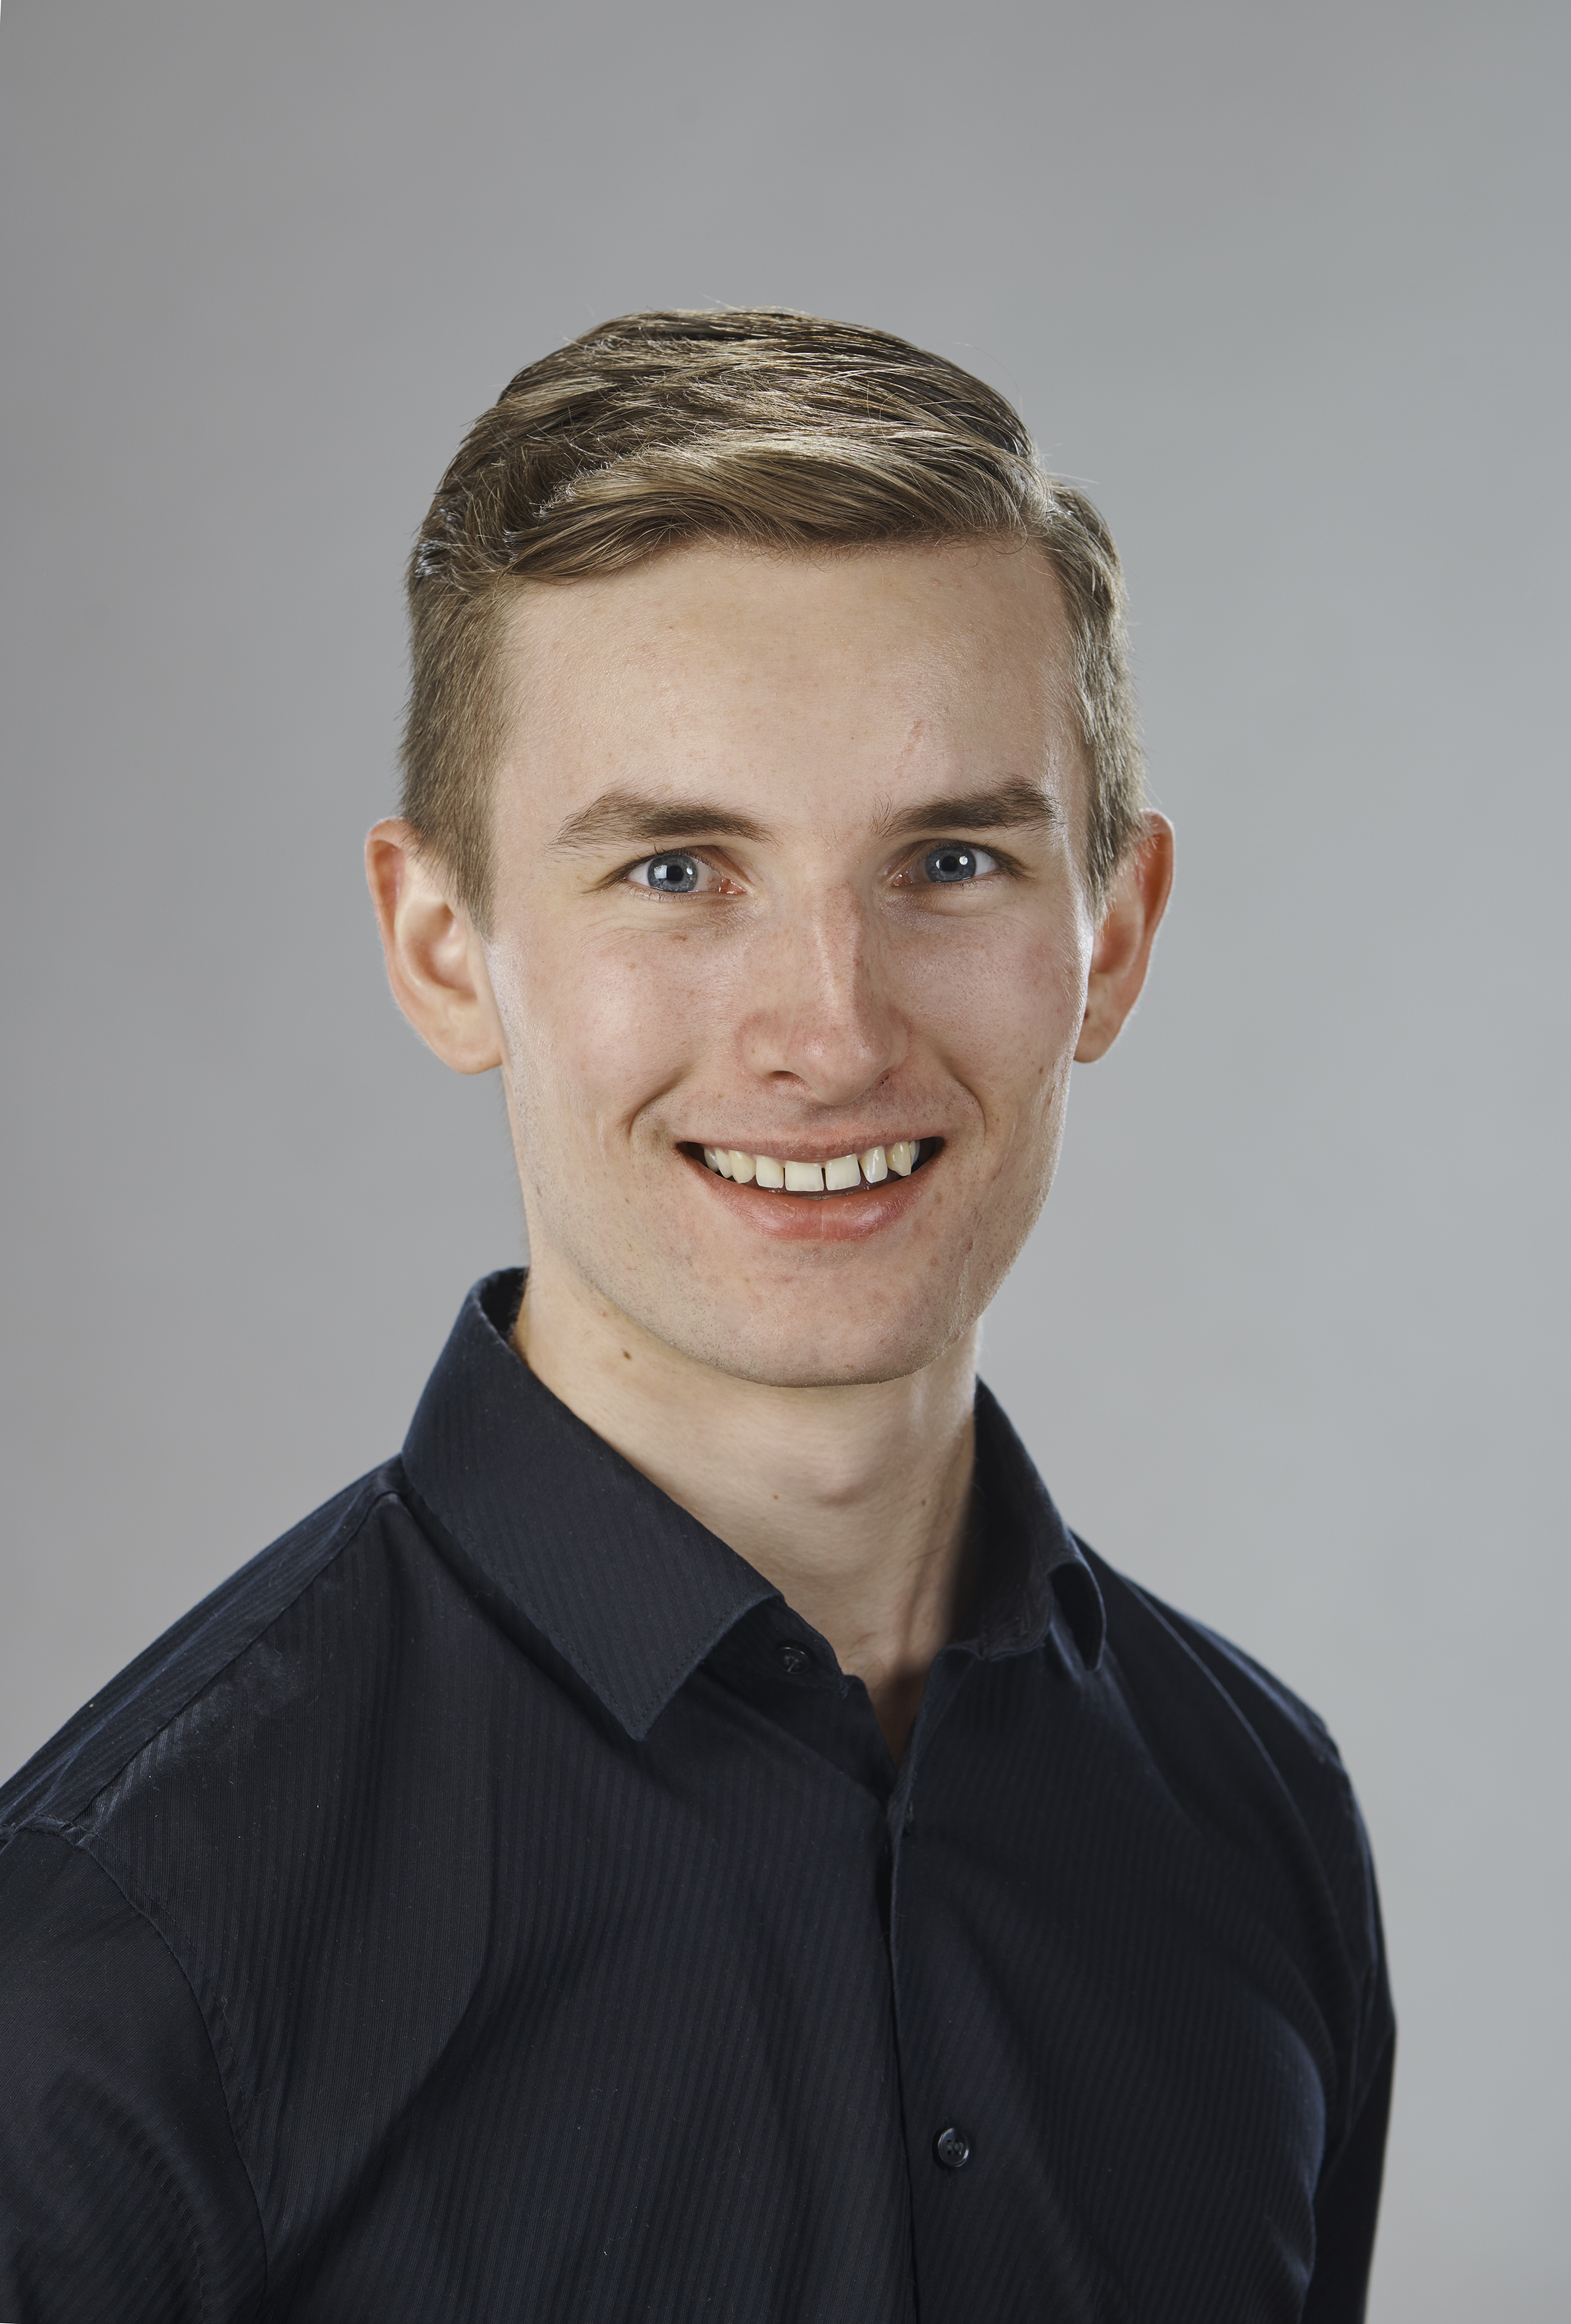
\includegraphics[width=0.9\linewidth,]{../figures/thilo_neu.jpg}

%----------------------------------------------------------------------------------------
%
%       CONTACT SECTION
%
%----------------------------------------------------------------------------------------

\begin{metasection}{Kontakt}

        \icontext{MapMarker}{12}{Voltastr. 65, 90459 Nürnberg}{black}\\[6pt]
        \icontext{MobilePhone}{12}{+49 160 45 72 775}{black}\\[6pt]
        \icontext{Send}{12}{business@thilo-wendt.de}{black}\\[6pt]

\end{metasection}

%----------------------------------------------------------------------------------------
%       META SECTION
%----------------------------------------------------------------------------------------

\begin{metasection}{Programmiersprachen}

%\icontext{Circle}{12}{C}{black}

  \begin{tabular*}{0.9\linewidth}[c]{rl}
    \faCode \space C & \textcolor{complcol}{\faCircle \space\space \faCircle \space\space
        \faCircle \space\space \faCircle \space\space \faCircleO} \\
    \faCode \space C++ & \textcolor{complcol}{\faCircle \space\space \faCircle \space\space
        \faCircle \space\space \faCircleO \space\space \faCircleO} \\
    \faCode \space VHDL  & \textcolor{complcol}{\faCircle \space\space \faCircle \space\space
        \faCircle \space\space \faCircleO \space\space \faCircleO} \\
    HTML \& CSS & \textcolor{complcol}{\faCircle \space\space \faCircle \space\space
        \faCircleO \space\space \faCircleO \space\space \faCircleO} \\
    \faDatabase \space SQL & \textcolor{complcol}{\faCircle \space\space \faCircle \space\space
        \faCircleO \space\space \faCircleO \space\space \faCircleO} \\
    Simatic S7  & \textcolor{complcol}{\faCircle \space\space \faCircle \space\space
        \faCircleO \space\space \faCircleO \space\space \faCircleO} \\
  \end{tabular*}




\end{metasection}

\begin{metasection}{Tools}

\faFlash \space Altium Designer, KiCAD und EAGLE \\
\textcolor{complcol}{\faCircle \space\space \faCircle \space\space
        \faCircle \space\space \faCircleO \space\space \faCircleO} \\[6pt]
\faCodeFork \space git \\
\textcolor{complcol}{\faCircle \space\space \faCircle \space\space
        \faCircle \space\space \faCircle \space\space \faCircleO} \\[6pt]

\faCubes \space Docker \\
\textcolor{complcol}{\faCircle \space\space \faCircle \space\space
        \faCircle \space\space \faCircle \space\space \faCircleO} \\[6pt]

\faTerminal \space Terminal (Linux and Mac) \\
\textcolor{complcol}{\faCircle \space\space \faCircle \space\space
        \faCircle \space\space \faCircle \space\space \faCircleO}

\end{metasection}

\begin{metasection}{Sprachen}

Deutsch (Muttersprache) \\
\textcolor{complcol}{\faCircle \space\space \faCircle \space\space
        \faCircle \space\space \faCircle \space\space \faCircle} \\[6pt]

Englisch \\
\textcolor{complcol}{\faCircle \space\space \faCircle \space\space
        \faCircle \space\space \faCircleO \space\space \faCircleO} \\[6pt]

Französisch \\
\textcolor{complcol}{\faCircle \space\space \faCircle \space\space
        \faCircleO \space\space \faCircleO \space\space \faCircleO}


\end{metasection}

%---------------------------------------------------------------------------------------
%       QR CODE (optional)
%----------------------------------------------------------------------------------------

%\vspace{12pt}
%\begin{center}
%\includegraphics[width=0.35\mpwidth]{qrcode}
%\end{center}

\end{minipage}}
\fcolorbox{white}{white}{\begin{minipage}[r][0.7\textheight][t]{0.69\linewidth}

%---------------------------------------------------------------------------------------
%       TITLE HEADLINE
%----------------------------------------------------------------------------------------
\vspace{-107pt}
% use this for multiple words like working titles etc.
% \hspace{-0.25\linewidth}\colorbox{bgcol}{\makebox[1.5\linewidth][c]{\hspace{46pt}\HUGE{\textcolor{white}{\uppercase{M.Sc. Jan Küster}} } \textcolor{sectcol}{\rule[-1mm]{1mm}{0.9cm}} \parbox[b]{5cm}{   \large{ \textcolor{white}{{IT Consultant}}}\\
%  \large{ \textcolor{white}{{JS Fullstack Engineer}}}}
% }}

% use this for single words, e.g. CV or RESUME etc.
\colorbox{bgcol}{\makebox[\mpwidth][c]{\huge{\textcolor{white}{\uppercase{Thilo Wendt}} } \textcolor{sectcol}{\rule[-1mm]{1mm}{0.7cm}} \huge{\textcolor{white}{\uppercase{Lebenslauf}} } }}

%----------------------------------------------------------------------------------------
%       HEADER IMAGE
%----------------------------------------------------------------------------------------


%\hspace{-1.6cm}
%\includegraphics[trim= 0 250 0 270,clip,width=1\linewidth+3.1cm]{myfoto.jpg}   %trimming relative to image size!
%\includegraphics[trim= 350 150 0 200, clip ,width=\linewidth]{myfoto.jpg}       %trimming relative to image size

%---------------------------------------------------------------------------------------
%       SUMMARY
%----------------------------------------------------------------------------------------

%============================================================================%
%
%       CV SECTIONS AND EVENTS (MAIN CONTENT)
%
%============================================================================%

%---------------------------------------------------------------------------------------
%       EDUCATION SECTION
%--------------------------------------------------------------------------------------

% param 1:      event time i.e. 2014 or 2011-2014 etc.
% param 2:      event name (what did you do?)
% param 3:      institution (where did you work / study)
% param 4:      what was your position
% param 5:      some words about your contributions

\vspace{13pt}
\cvsection{Bildung}

\cvevent{Seit 10/2019}{Master Applied Research in Engineering
  Sciences}{TH-Nürnberg/Institut ELSYS}{Hardwareentwicklung für eine
  echtzeitfähige Berechnungsplattform}{Akademische Ausbildung im Bereich
System Engineering}

\cvevent{10/2019 - 06/2020}{Master Projekt: Entwicklung und Optimierung von
  Leiterplatten mit Altium Designer}{TH-Nürnberg/Institut ELSYS}{Entwicklung
  einer Erweiterungsplatine für eine echtzeitfähige
  Berechnungsplattform}{Revision des Mainboards einer echtzeitfähigen Berechnungsplattform}

\cvevent{10/2015 - 09/2019}{Abschluss B. Eng. Elektrotechnik und \newline
  Informationstechnik (1.6)}{TH-Nürnberg Georg Simon Ohm}{Bachelorarbeit:
  Entwicklung einer LED basierten Beleuchtungseinheit für Züge}{Schwerpunkt:
  System Design von eingebetteten Systemen und PCB-Entwicklung}

\cvevent{08/2015 - 08/2018}{Ausbildung zum Elektroniker für
  Automatisierungstechnik (IHK) (91 von 100 Punkten)}{Siemens}{Handwerkliche
  Ausbildung im Bereich Automatisierungstechnik}{Programmierung von Siemens
  Simatic S7 speicherprogrammierbare Steuerungen}

\cvevent{09/2010 - 07/2015}{Schule und Abitur (1.4)}{Gymnasium
  Isernhagen}{Abschluss mit Schwerpunkt Mathematik und
  Naturwissenschaften}{Engagement in verschiedenen Arbeitsgruppen z.B. Licht und
Ton für Theateraufführungen}

%---------------------------------------------------------------------------------------
%       EXPERIENCE
%----------------------------------------------------------------------------------------

\vspace{23pt}

\cvsection{Erfahrung}

\cvevent{10/2016 - 01/2018}{Studentisches Tutorium}{TH-Nürnberg Georg Simon
  Ohm}{Themen: Elektrische Messtechnik, Mikrocomputertechik, Grundlagen der
  Elektrotechnik}{Ausbau von Präsentationstechniken und Führungsqualitäten
  gegenüber Gruppen}

\cvevent{07/2017 - 07/2018}{Internationale Praktika im Bereich \newline
  Kraftwerksinbetriebnahme}{Siemens}{Praktikum in den VAE (2017) und in Ägypten
  (2018)}{Interkulturelle und fachliche Erfahrungen in außereuropäischen
  Kulturen}

\vspace{12pt}
\cvsection{Nebenprojekte}

 \begin{tabular*}{0.9\linewidth}[c]{m{0.05\linewidth} m{0.8\linewidth}}
   
\includegraphics[width=0.5cm]{../figures/tools.pdf} & Handwerkliche Projekte
                                                         im Bereich
                                                         Holzbearbeitung und
                                                         Fahrräder \\
   
\includegraphics[width=0.5cm]{../figures/cloud.pdf} & Aufbau und Wartung eines Docker
                                                         basierten Cloud Servers und einer
                                                         Online Community Infrastruktur
                                                         (Website, Forum und Wiki) \\
   
\includegraphics[width=0.5cm]{../figures/dumbbell-solid.pdf} & Leistungssport
                                                                  im Rudern (2010 -
                                                                  2019) seitdem
                                                                  Radfahren
                                                                  Laufen und
                                                                  Langlaufen \\
   
\includegraphics[width=0.5cm]{../figures/music.pdf} & Sänger und Bassist in verschiedenen
                                                         Bands (2010 - 2017) \\
\end{tabular*}

\end{minipage}}
%end of the colorbox 


%-------------------------------------------------------------------------------------------------
%       ARTIFICIAL FOOTER (fancy footer cannot exceed linewidth) 
%--------------------------------------------------------------------------------------------------

\null
\vspace*{\fill}
\hspace{-0.25\linewidth}\colorbox{bgcol}{\makebox[1.5\linewidth][c]{ \small \textcolor{white}{\today}}}

%============================================================================%
%
%
%
%       DOCUMENT END
%
%
%
%============================================================================%
\end{document}



%%% Local Variables:
%%% mode: latex
%%% TeX-master: t
%%% End:
